\FChapter{Chapter Twenty-Five}{25}

\Lettrine{T}{he} \textsc{month of courtship} had wasted: its very last hours were being
numbered.  There was no putting off the day that advanced---the bridal
day; and all preparations for its arrival were complete.  \emph{I}, at
least, had nothing more to do: there were my trunks, packed, locked,
corded, ranged in a row along the wall of my little chamber; to-morrow,
at this time, they would be far on their road to London: and so should I
\emph{(D.\,V.),}---or rather, not I, but one Jane Rochester, a person whom as yet
I knew not.  The cards of address alone remained to nail on: they lay,
four little squares, in the drawer.  \Mr{} Rochester had himself written
the direction, \enquote{\Mrs{} Rochester, --- Hotel, London,} on each: I
could not persuade myself to affix them, or to have them affixed.  \Mrs{}
Rochester!  She did not exist: she would not be born till to-morrow,
some time after eight o'clock \AM; and I would wait to be assured she
had come into the world alive before I assigned to her all that
property.  It was enough that in yonder closet, opposite my
dressing-table, garments said to be hers had already displaced my black
stuff Lowood frock and straw bonnet: for not to me appertained that suit
of wedding raiment; the pearl-coloured robe, the vapoury veil pendent
from the usurped portmanteau.  I shut the closet to conceal the strange,
wraith-like apparel it contained; which, at this evening hour---nine
o'clock---gave out certainly a most ghostly shimmer through the shadow
of my apartment.  \enquote{I will leave you by yourself, white dream,} I
said.  \enquote{I am feverish: I hear the wind blowing: I will go out of
	doors and feel it.}

It was not only the hurry of preparation that made me feverish; not only
the anticipation of the great change---the new life which was to
commence to-morrow: both these circumstances had their share, doubtless,
in producing that restless, excited mood which hurried me forth at this
late hour into the darkening grounds: but a third cause influenced my
mind more than they.

I had at heart a strange and anxious thought.  Something had happened
which I could not comprehend; no one knew of or had seen the event but
myself: it had taken place the preceding night.  \Mr{} Rochester that
night was absent from home; nor was he yet returned: business had called
him to a small estate of two or three farms he possessed thirty miles
off---business it was requisite he should settle in person, previous to
his meditated departure from England.  I waited now his return; eager to
disburthen my mind, and to seek of him the solution of the enigma that
perplexed me.  Stay till he comes, reader; and, when I disclose my
secret to him, you shall share the confidence.

I sought the orchard, driven to its shelter by the wind, which all day
had blown strong and full from the south, without, however, bringing a
speck of rain.  Instead of subsiding as night drew on, it seemed to
augment its rush and deepen its roar: the trees blew steadfastly one
way, never writhing round, and scarcely tossing back their boughs once
in an hour; so continuous was the strain bending their branchy heads
northward---the clouds drifted from pole to pole, fast following, mass
on mass: no glimpse of blue sky had been visible that July day.

It was not without a certain wild pleasure I ran before the wind,
delivering my trouble of mind to the measureless air-torrent thundering
through space.  Descending the laurel walk, I faced the wreck of the
chestnut-tree; it stood up black and riven: the trunk, split down the
centre, gasped ghastly.  The cloven halves were not broken from each
other, for the firm base and strong roots kept them unsundered below;
though community of vitality was destroyed---the sap could flow no more:
their great boughs on each side were dead, and next winter's tempests
would be sure to fell one or both to earth: as yet, however, they might
be said to form one tree---a ruin, but an entire ruin.

\enquote{You did right to hold fast to each other,} I said: as if the
monster-splinters were living things, and could hear me.  \enquote{I
	think, scathed as you look, and charred and scorched, there must be a
	little sense of life in you yet, rising out of that adhesion at the
	faithful, honest roots: you will never have green leaves more---never
	more see birds making nests and singing idyls in your boughs; the time
	of pleasure and love is over with you: but you are not desolate: each of
	you has a comrade to sympathise with him in his decay.}  As I looked up
at them, the moon appeared momentarily in that part of the sky which
filled their fissure; her disk was blood-red and half overcast; she
seemed to throw on me one bewildered, dreary glance, and buried herself
again instantly in the deep drift of cloud.  The wind fell, for a
second, round Thornfield; but far away over wood and water, poured a
wild, melancholy wail: it was sad to listen to, and I ran off again.

Here and there I strayed through the orchard, gathered up the apples
with which the grass round the tree roots was thickly strewn; then I
employed myself in dividing the ripe from the unripe; I carried them
into the house and put them away in the store-room.  Then I repaired to
the library to ascertain whether the fire was lit, for, though summer, I
knew on such a gloomy evening \Mr{} Rochester would like to see a cheerful
hearth when he came in: yes, the fire had been kindled some time, and
burnt well.  I placed his arm-chair by the chimney-corner: I wheeled the
table near it: I let down the curtain, and had the candles brought in
ready for lighting.  More restless than ever, when I had completed these
arrangements I could not sit still, nor even remain in the house: a
little time-piece in the room and the old clock in the hall
simultaneously struck ten.

\enquote{How late it grows!} I said.  \enquote{I will run down to the
	gates: it is moonlight at intervals; I can see a good way on the road.
	He may be coming now, and to meet him will save some minutes of
	suspense.}

The wind roared high in the great trees which embowered the gates; but
the road as far as I could see, to the right hand and the left, was all
still and solitary: save for the shadows of clouds crossing it at
intervals as the moon looked out, it was but a long pale line, unvaried
by one moving speck.

A puerile tear dimmed my eye while I looked---a tear of disappointment
and impatience; ashamed of it, I wiped it away.  I lingered; the moon
shut herself wholly within her chamber, and drew close her curtain of
dense cloud: the night grew dark; rain came driving fast on the gale.

\enquote{I wish he would come!  I wish he would come!} I exclaimed,
seized with hypochondriac foreboding.  I had expected his arrival before
tea; now it was dark: what could keep him?  Had an accident happened?
The event of last night again recurred to me.  I interpreted it as a
warning of disaster.  I feared my hopes were too bright to be realised;
and I had enjoyed so much bliss lately that I imagined my fortune had
passed its meridian, and must now decline.

\enquote{Well, I cannot return to the house,} I thought; \enquote{I
	cannot sit by the fireside, while he is abroad in inclement weather:
	better tire my limbs than strain my heart; I will go forward and meet
	him.}

I set out; I walked fast, but not far: ere I had measured a quarter of a
mile, I heard the tramp of hoofs; a horseman came on, full gallop; a dog
ran by his side.  Away with evil presentiment!  It was he: here he was,
mounted on Mesrour, followed by Pilot.  He saw me; for the moon had
opened a blue field in the sky, and rode in it watery bright: he took
his hat off, and waved it round his head.  I now ran to meet him.

\enquote{There!} he exclaimed, as he stretched out his hand and bent
from the saddle: \enquote{You can't do without me, that is evident.
	Step on my boot-toe; give me both hands: mount!}

I obeyed: joy made me agile: I sprang up before him.  A hearty kissing I
got for a welcome, and some boastful triumph, which I swallowed as well
as I could.  He checked himself in his exultation to demand,
\enquote{But is there anything the matter, Janet, that you come to meet
	me at such an hour?  Is there anything wrong?}

\enquote{No, but I thought you would never come.  I could not bear to
	wait in the house for you, especially with this rain and wind.}

\enquote{Rain and wind, indeed!  Yes, you are dripping like a mermaid;
	pull my cloak round you: but I think you are feverish, Jane: both your
	cheek and hand are burning hot.  I ask again, is there anything the
	matter?}

\enquote{Nothing now; I am neither afraid nor unhappy.}

\enquote{Then you have been both?}

\enquote{Rather: but I'll tell you all about it by-and-bye, sir; and I
	daresay you will only laugh at me for my pains.}

\enquote{I'll laugh at you heartily when to-morrow is past; till then I
	dare not: my prize is not certain.  This is you, who have been as
	slippery as an eel this last month, and as thorny as a briar-rose?  I
	could not lay a finger anywhere but I was pricked; and now I seem to
	have gathered up a stray lamb in my arms.  You wandered out of the fold
	to seek your shepherd, did you, Jane?}

\enquote{I wanted you: but don't boast.  Here we are at Thornfield: now
	let me get down.}

He landed me on the pavement.  As John took his horse, and he followed
me into the hall, he told me to make haste and put something dry on, and
then return to him in the library; and he stopped me, as I made for the
staircase, to extort a promise that I would not be long: nor was I long;
in five minutes I rejoined him.  I found him at supper.

\enquote{Take a seat and bear me company, Jane: please God, it is the
	last meal but one you will eat at Thornfield Hall for a long time.}

I sat down near him, but told him I could not eat.  \enquote{Is it
	because you have the prospect of a journey before you, Jane?  Is it the
	thoughts of going to London that takes away your appetite?}

\enquote{I cannot see my prospects clearly to-night, sir; and I hardly
	know what thoughts I have in my head.  Everything in life seems unreal.}

\enquote{Except me: I am substantial enough---touch me.}

\enquote{You, sir, are the most phantom-like of all: you are a mere
	dream.}

He held out his hand, laughing.  \enquote{Is that a dream?} said he,
placing it close to my eyes.  He had a rounded, muscular, and vigorous
hand, as well as a long, strong arm.

\enquote{Yes; though I touch it, it is a dream,} said I, as I put it
down from before my face.  \enquote{Sir, have you finished supper?}

\enquote{Yes, Jane.}

I rang the bell and ordered away the tray.  When we were again alone, I
stirred the fire, and then took a low seat at my master's knee.

\enquote{It is near midnight,} I said.

\enquote{Yes: but remember, Jane, you promised to wake with me the night
	before my wedding.}

\enquote{I did; and I will keep my promise, for an hour or two at least:
	I have no wish to go to bed.}

\enquote{Are all your arrangements complete?}

\enquote{All, sir.}

\enquote{And on my part likewise,} he returned, \enquote{I have settled
	everything; and we shall leave Thornfield to-morrow, within half-an-hour
	after our return from church.}

\enquote{Very well, sir.}

\enquote{With what an extraordinary smile you uttered that word---\enquote{very
		well,} Jane!  What a bright spot of colour you have on each cheek! and
	how strangely your eyes glitter!  Are you well?}

\enquote{I believe I am.}

\enquote{Believe!  What is the matter?  Tell me what you feel.}

\enquote{I could not, sir: no words could tell you what I feel.  I wish
	this present hour would never end: who knows with what fate the next may
	come charged?}

\enquote{This is hypochondria, Jane.  You have been over-excited, or
	over-fatigued.}

\enquote{Do you, sir, feel calm and happy?}

\enquote{Calm?---no: but happy---to the heart's core.}

I looked up at him to read the signs of bliss in his face: it was ardent
and flushed.

\enquote{Give me your confidence, Jane,} he said: \enquote{relieve your
	mind of any weight that oppresses it, by imparting it to me.  What do
	you fear?---that I shall not prove a good husband?}

\enquote{It is the idea farthest from my thoughts.}

\enquote{Are you apprehensive of the new sphere you are about to
	enter?---of the new life into which you are passing?}

\enquote{No.}

\enquote{You puzzle me, Jane: your look and tone of sorrowful audacity
	perplex and pain me.  I want an explanation.}

\enquote{Then, sir, listen.  You were from home last night?}

\enquote{I was: I know that; and you hinted a while ago at something
	which had happened in my absence:---nothing, probably, of consequence;
	but, in short, it has disturbed you.  Let me hear it.  \Mrs{} Fairfax has
	said something, perhaps? or you have overheard the servants talk?---your
	sensitive self-respect has been wounded?}

\enquote{No, sir.}  It struck twelve---I waited till the time-piece had
concluded its silver chime, and the clock its hoarse, vibrating stroke,
and then I proceeded.

\enquote{All day yesterday I was very busy, and very happy in my ceaseless
	bustle; for I am not, as you seem to think, troubled by any haunting
	fears about the new sphere, et cetera: I think it a glorious thing to
	have the hope of living with you, because I love you.  No, sir, don't
	caress me now---let me talk undisturbed.  Yesterday I trusted well in
	Providence, and believed that events were working together for your good
	and mine: it was a fine day, if you recollect---the calmness of the air
	and sky forbade apprehensions respecting your safety or comfort on your
	journey.  I walked a little while on the pavement after tea, thinking of
	you; and I beheld you in imagination so near me, I scarcely missed your
	actual presence.  I thought of the life that lay before me---\emph{your}
	life, sir---an existence more expansive and stirring than my own: as
	much more so as the depths of the sea to which the brook runs are than
	the shallows of its own strait channel.  I wondered why moralists call
	this world a dreary wilderness: for me it blossomed like a rose.  Just
	at sunset, the air turned cold and the sky cloudy: I went in, Sophie
	called me upstairs to look at my wedding-dress, which they had just
	brought; and under it in the box I found your present---the veil which,
	in your princely extravagance, you sent for from London: resolved, I
	suppose, since I would not have jewels, to cheat me into accepting
	something as costly.  I smiled as I unfolded it, and devised how I would
	tease you about your aristocratic tastes, and your efforts to masque
	your plebeian bride in the attributes of a peeress.  I thought how I
	would carry down to you the square of unembroidered blond I had myself
	prepared as a covering for my low-born head, and ask if that was not
	good enough for a woman who could bring her husband neither fortune,
	beauty, nor connections.  I saw plainly how you would look; and heard
	your impetuous republican answers, and your haughty disavowal of any
	necessity on your part to augment your wealth, or elevate your standing,
	by marrying either a purse or a coronet.}

\enquote{How well you read me, you witch!} interposed \Mr{} Rochester:
\enquote{but what did you find in the veil besides its embroidery?  Did
	you find poison, or a dagger, that you look so mournful now?}

\enquote{No, no, sir; besides the delicacy and richness of the fabric, I
	found nothing save Fairfax Rochester's pride; and that did not scare me,
	because I am used to the sight of the demon.  But, sir, as it grew dark,
	the wind rose: it blew yesterday evening, not as it blows now---wild and
	high---but \enquote{with a sullen, moaning sound} far more eerie.  I
	wished you were at home.  I came into this room, and the sight of the
	empty chair and fireless hearth chilled me.  For some time after I went
	to bed, I could not sleep---a sense of anxious excitement distressed
	me.  The gale still rising, seemed to my ear to muffle a mournful
	under-sound; whether in the house or abroad I could not at first tell,
	but it recurred, doubtful yet doleful at every lull; at last I made out
	it must be some dog howling at a distance.  I was glad when it ceased.
	On sleeping, I continued in dreams the idea of a dark and gusty night.
	I continued also the wish to be with you, and experienced a strange,
	regretful consciousness of some barrier dividing us.  During all my
	first sleep, I was following the windings of an unknown road; total
	obscurity environed me; rain pelted me; I was burdened with the charge
	of a little child: a very small creature, too young and feeble to walk,
	and which shivered in my cold arms, and wailed piteously in my ear.  I
	thought, sir, that you were on the road a long way before me; and I
	strained every nerve to overtake you, and made effort on effort to utter
	your name and entreat you to stop---but my movements were fettered, and
	my voice still died away inarticulate; while you, I felt, withdrew
	farther and farther every moment.}

\enquote{And these dreams weigh on your spirits now, Jane, when I am close to
	you?  Little nervous subject!  Forget visionary woe, and think only of
	real happiness!  You say you love me, Janet: yes---I will not forget
	that; and you cannot deny it.  \emph{Those} words did not die
	inarticulate on your lips.  I heard them clear and soft: a thought too
	solemn perhaps, but sweet as music---\enquote{I think it is a glorious thing to
		have the hope of living with you, Edward, because I love you.}  Do you
	love me, Jane?---repeat it.}

\enquote{I do, sir---I do, with my whole heart.}

\enquote{Well,} he said, after some minutes' silence, \enquote{it is
	strange; but that sentence has penetrated my breast painfully.  Why?  I
	think because you said it with such an earnest, religious energy, and
	because your upward gaze at me now is the very sublime of faith, truth,
	and devotion: it is too much as if some spirit were near me.  Look
	wicked, Jane: as you know well how to look: coin one of your wild, shy,
	provoking smiles; tell me you hate me---tease me, vex me; do anything
	but move me: I would rather be incensed than saddened.}

\enquote{I will tease you and vex you to your heart's content, when I
	have finished my tale: but hear me to the end.}

\enquote{I thought, Jane, you had told me all.  I thought I had found
	the source of your melancholy in a dream.}

I shook my head.  \enquote{What! is there more?  But I will not believe
	it to be anything important.  I warn you of incredulity beforehand.  Go
	on.}

The disquietude of his air, the somewhat apprehensive impatience of his
manner, surprised me: but I proceeded.

\enquote{I dreamt another dream, sir: that Thornfield Hall was a dreary
	ruin, the retreat of bats and owls.  I thought that of all the stately
	front nothing remained but a shell-like wall, very high and very
	fragile-looking.  I wandered, on a moonlight night, through the
	grass-grown enclosure within: here I stumbled over a marble hearth, and
	there over a fallen fragment of cornice.  Wrapped up in a shawl, I still
	carried the unknown little child: I might not lay it down anywhere,
	however tired were my arms---however much its weight impeded my
	progress, I must retain it.  I heard the gallop of a horse at a distance
	on the road; I was sure it was you; and you were departing for many
	years and for a distant country.  I climbed the thin wall with frantic
	perilous haste, eager to catch one glimpse of you from the top: the
	stones rolled from under my feet, the ivy branches I grasped gave way,
	the child clung round my neck in terror, and almost strangled me; at
	last I gained the summit.  I saw you like a speck on a white track,
	lessening every moment.  The blast blew so strong I could not stand.  I
	sat down on the narrow ledge; I hushed the scared infant in my lap: you
	turned an angle of the road: I bent forward to take a last look; the
	wall crumbled; I was shaken; the child rolled from my knee, I lost my
	balance, fell, and woke.}

\enquote{Now, Jane, that is all.}

\enquote{All the preface, sir; the tale is yet to come.  On waking, a
	gleam dazzled my eyes; I thought---Oh, it is daylight!  But I was
	mistaken; it was only candlelight.  Sophie, I supposed, had come in.
	There was a light in the dressing-table, and the door of the closet,
	where, before going to bed, I had hung my wedding-dress and veil, stood
	open; I heard a rustling there.  I asked, \enquote{Sophie, what are you
		doing?}  No one answered; but a form emerged from the closet; it took
	the light, held it aloft, and surveyed the garments pendent from the
	portmanteau.  \enquote{Sophie!  Sophie!}  I again cried: and still it
	was silent.  I had risen up in bed, I bent forward: first surprise, then
	bewilderment, came over me; and then my blood crept cold through my
	veins.  \Mr{} Rochester, this was not Sophie, it was not Leah, it was not
	\Mrs{} Fairfax: it was not---no, I was sure of it, and am still---it was
	not even that strange woman, Grace Poole.}

\enquote{It must have been one of them,} interrupted my master.

\enquote{No, sir, I solemnly assure you to the contrary.  The shape
	standing before me had never crossed my eyes within the precincts of
	Thornfield Hall before; the height, the contour were new to me.}

\enquote{Describe it, Jane.}

\enquote{It seemed, sir, a woman, tall and large, with thick and dark
	hair hanging long down her back.  I know not what dress she had on: it
	was white and straight; but whether gown, sheet, or shroud, I cannot
	tell.}

\enquote{Did you see her face?}

\enquote{Not at first.  But presently she took my veil from its place;
	she held it up, gazed at it long, and then she threw it over her own
	head, and turned to the mirror.  At that moment I saw the reflection of
	the visage and features quite distinctly in the dark oblong glass.}

\enquote{And how were they?}

\enquote{Fearful and ghastly to me---oh, sir, I never saw a face like
	it!  It was a discoloured face---it was a savage face.  I wish I could
	forget the roll of the red eyes and the fearful blackened inflation of
	the lineaments!}

\enquote{Ghosts are usually pale, Jane.}

\enquote{This, sir, was purple: the lips were swelled and dark; the brow
	furrowed: the black eyebrows widely raised over the bloodshot eyes.
	Shall I tell you of what it reminded me?}

\enquote{You may.}

\enquote{Of the foul German spectre---the Vampyre.}

\enquote{Ah!---what did it do?}

\enquote{Sir, it removed my veil from its gaunt head, rent it in two
	parts, and flinging both on the floor, trampled on them.}

\begin{figure}
	\begin{sidecaption}{\enquote{It removed my veil\linebreak from its gaunt head,\linebreak rent it in two parts,\linebreak and flinging both\linebreak on the floor,\linebreak trampled on them.}}[p272b]
		\centering
		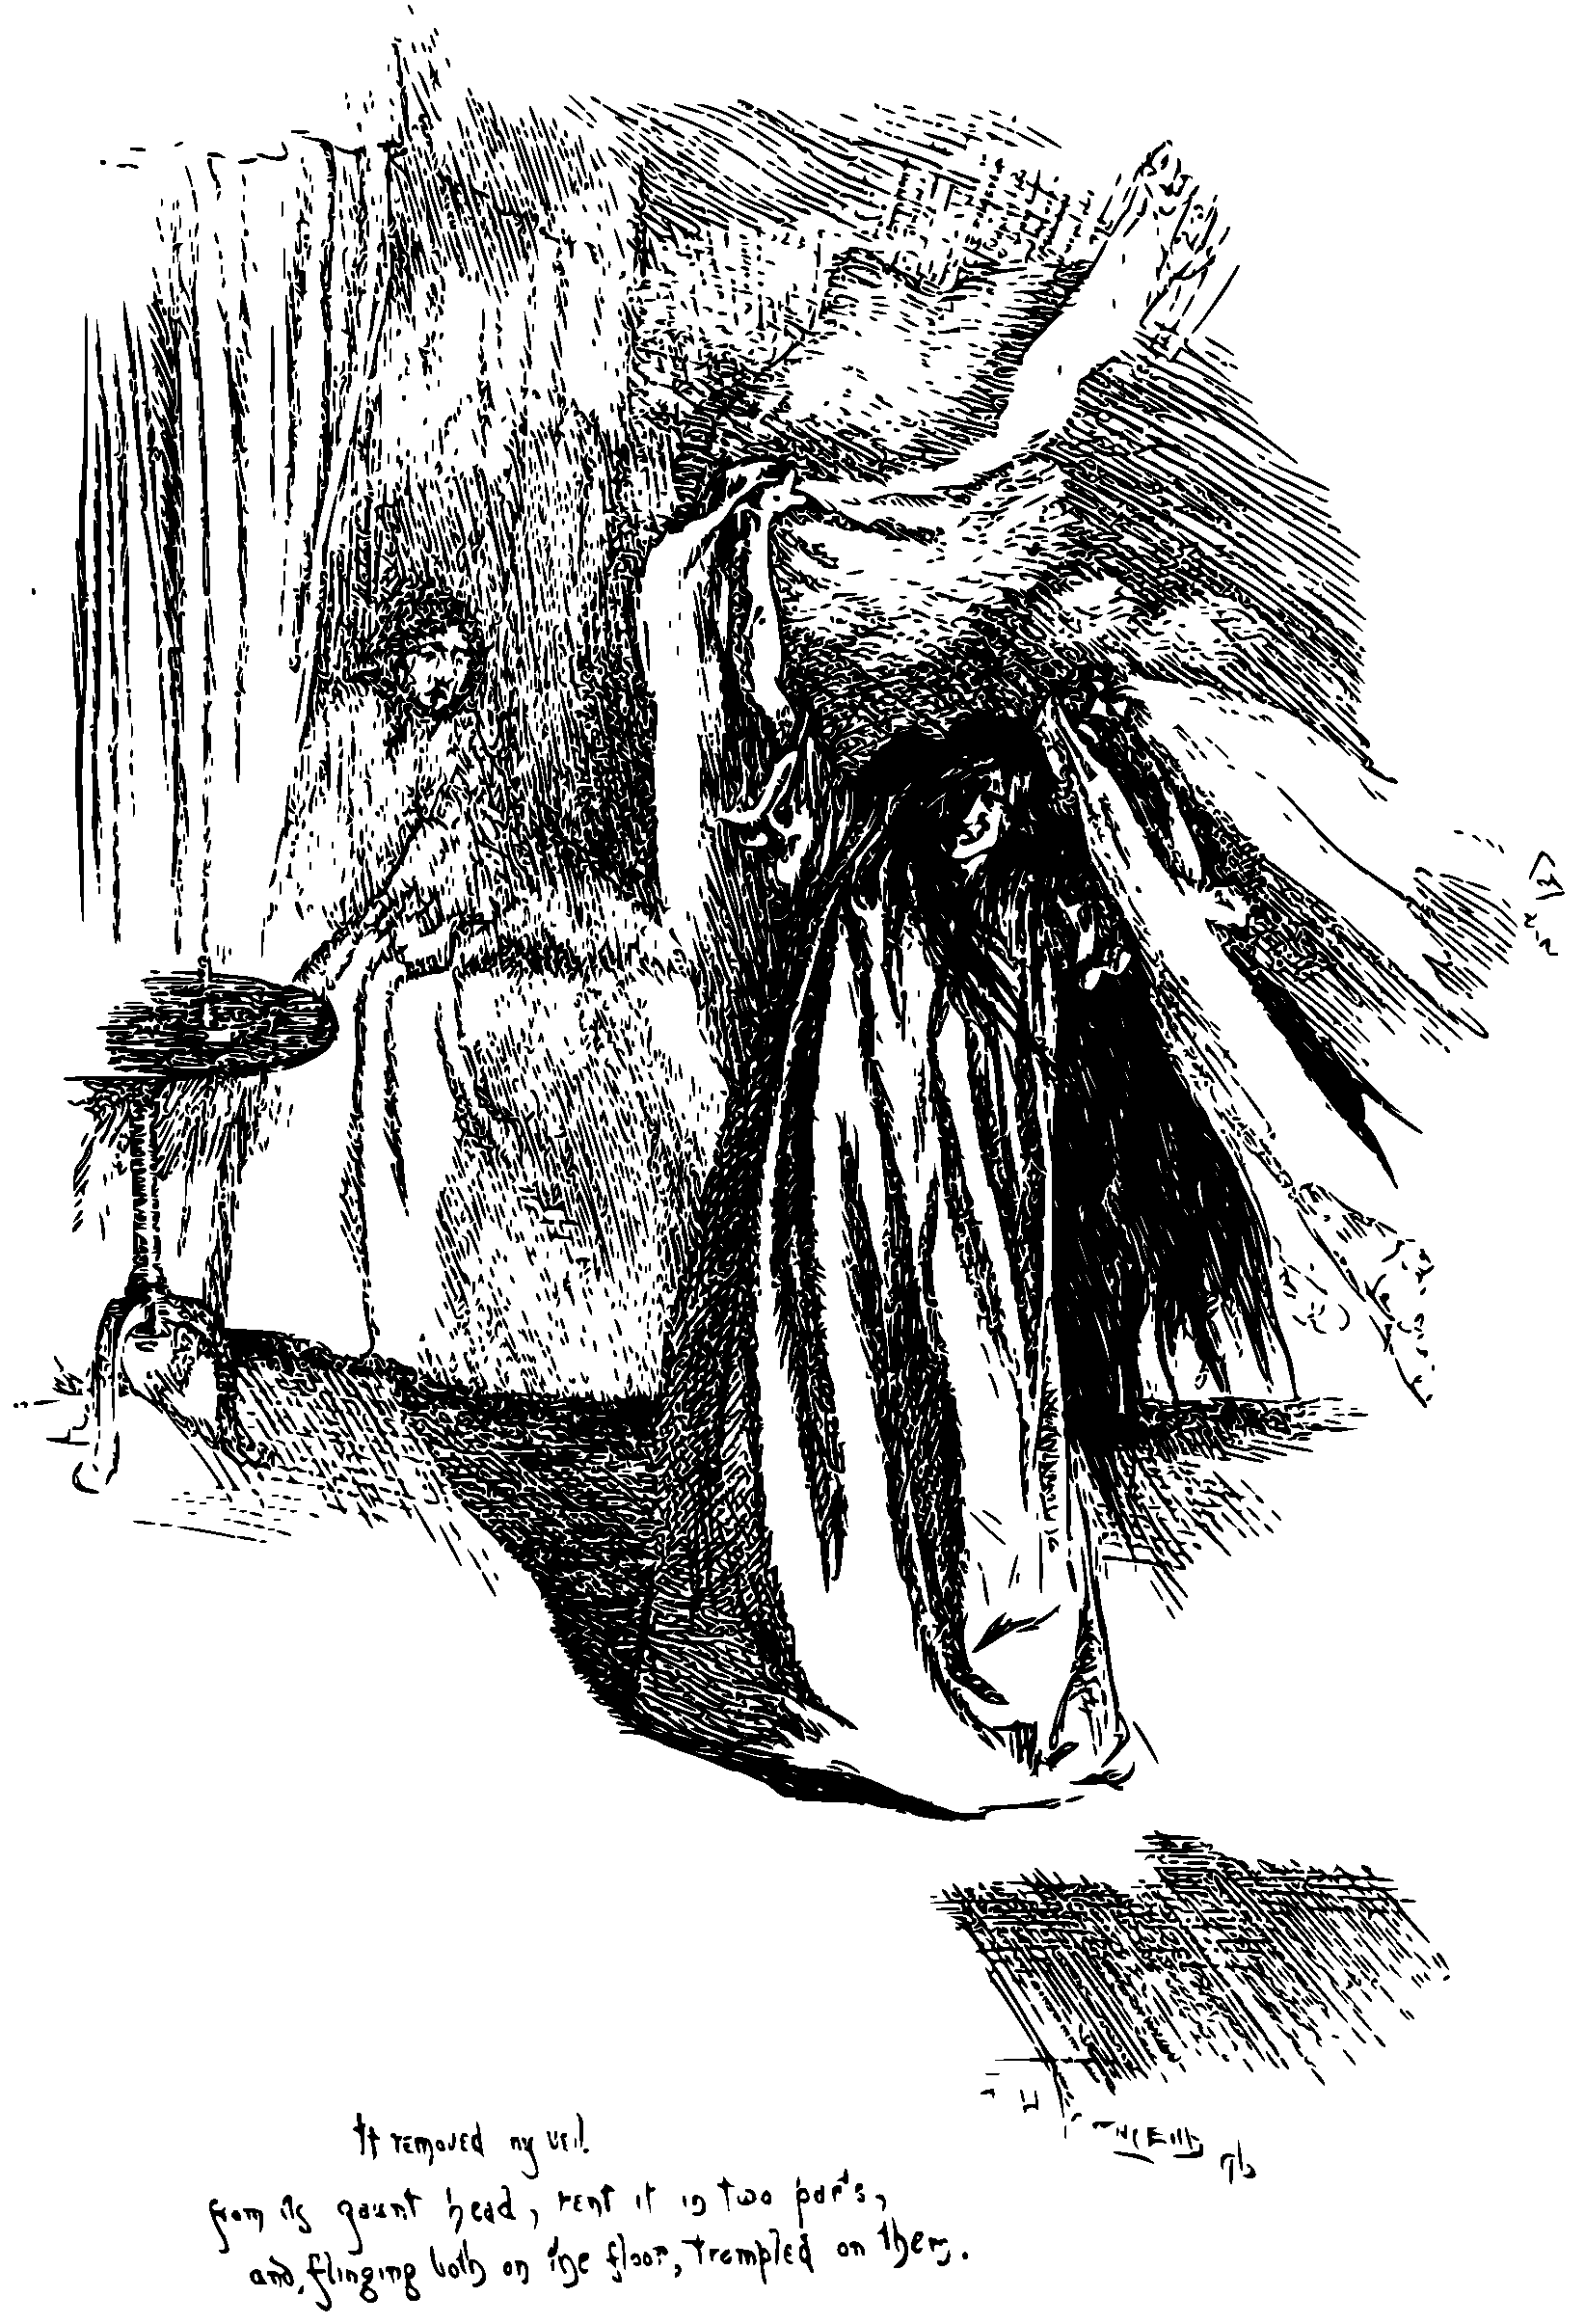
\includegraphics[width=\linewidth]{images/p272b.pdf}
	\end{sidecaption}
\end{figure}

\enquote{Afterwards?}

\enquote{It drew aside the window-curtain and looked out; perhaps it saw
	dawn approaching, for, taking the candle, it retreated to the door.
	Just at my bedside, the figure stopped: the fiery eyes glared upon
	me---she thrust up her candle close to my face, and extinguished it
	under my eyes.  I was aware her lurid visage flamed over mine, and I
	lost consciousness: for the second time in my life---only the second
	time---I became insensible from terror.}

\enquote{Who was with you when you revived?}

\enquote{No one, sir, but the broad day.  I rose, bathed my head and
	face in water, drank a long draught; felt that though enfeebled I was
	not ill, and determined that to none but you would I impart this
	vision.  Now, sir, tell me who and what that woman was?}

\enquote{The creature of an over-stimulated brain; that is certain.  I
	must be careful of you, my treasure: nerves like yours were not made for
	rough handling.}

\enquote{Sir, depend on it, my nerves were not in fault; the thing was
	real: the transaction actually took place.}

\enquote{And your previous dreams, were they real too?  Is Thornfield
	Hall a ruin?  Am I severed from you by insuperable obstacles?  Am I
	leaving you without a tear---without a kiss---without a word?}

\enquote{Not yet.}

\enquote{Am I about to do it?  Why, the day is already commenced which
	is to bind us indissolubly; and when we are once united, there shall be
	no recurrence of these mental terrors: I guarantee that.}

\enquote{Mental terrors, sir!  I wish I could believe them to be only
	such: I wish it more now than ever; since even you cannot explain to me
	the mystery of that awful visitant.}

\enquote{And since I cannot do it, Jane, it must have been unreal.}

\enquote{But, sir, when I said so to myself on rising this morning, and
	when I looked round the room to gather courage and comfort from the
	cheerful aspect of each familiar object in full daylight, there---on the
	carpet---I saw what gave the distinct lie to my hypothesis,---the veil,
	torn from top to bottom in two halves!}

I felt \Mr{} Rochester start and shudder; he hastily flung his arms round
me.  \enquote{Thank God!} he exclaimed, \enquote{that if anything
	malignant did come near you last night, it was only the veil that was
	harmed.  Oh, to think what might have happened!}

He drew his breath short, and strained me so close to him, I could
scarcely pant.  After some minutes' silence, he continued, cheerily---

\enquote{Now, Janet, I'll explain to you all about it.  It was half
	dream, half reality.  A woman did, I doubt not, enter your room: and
	that woman was---must have been---Grace Poole.  You call her a strange
	being yourself: from all you know, you have reason so to call her---what
	did she do to me? what to Mason?  In a state between sleeping and
	waking, you noticed her entrance and her actions; but feverish, almost
	delirious as you were, you ascribed to her a goblin appearance different
	from her own: the long dishevelled hair, the swelled black face, the
	exaggerated stature, were figments of imagination; results of nightmare:
	the spiteful tearing of the veil was real: and it is like her.  I see
	you would ask why I keep such a woman in my house: when we have been
	married a year and a day, I will tell you; but not now.  Are you
	satisfied, Jane?  Do you accept my solution of the mystery?}

I reflected, and in truth it appeared to me the only possible one:
satisfied I was not, but to please him I endeavoured to appear
so---relieved, I certainly did feel; so I answered him with a contented
smile.  And now, as it was long past one, I prepared to leave him.

\enquote{Does not Sophie sleep with Adèle in the nursery?} he asked, as
I lit my candle.

\enquote{Yes, sir.}

\enquote{And there is room enough in Adèle's little bed for you.  You
	must share it with her to-night, Jane: it is no wonder that the incident
	you have related should make you nervous, and I would rather you did not
	sleep alone: promise me to go to the nursery.}

\enquote{I shall be very glad to do so, sir.}

\enquote{And fasten the door securely on the inside.  Wake Sophie when
	you go upstairs, under pretence of requesting her to rouse you in good
	time to-morrow; for you must be dressed and have finished breakfast
	before eight.  And now, no more sombre thoughts: chase dull care away,
	Janet.  Don't you hear to what soft whispers the wind has fallen? and
	there is no more beating of rain against the window-panes: look here}
(he lifted up the curtain)---\enquote{it is a lovely night!}

It was.  Half heaven was pure and stainless: the clouds, now trooping
before the wind, which had shifted to the west, were filing off eastward
in long, silvered columns.  The moon shone peacefully.

\enquote{Well,} said \Mr{} Rochester, gazing inquiringly into my eyes,
\enquote{how is my Janet now?}

\enquote{The night is serene, sir; and so am I\@.}

\enquote{And you will not dream of separation and sorrow to-night; but
	of happy love and blissful union.}

This prediction was but half fulfilled: I did not indeed dream of
sorrow, but as little did I dream of joy; for I never slept at all.
With little Adèle in my arms, I watched the slumber of childhood---so
tranquil, so passionless, so innocent---and waited for the coming day:
all my life was awake and astir in my frame: and as soon as the sun rose
I rose too.  I remember Adèle clung to me as I left her: I remember I
kissed her as I loosened her little hands from my neck; and I cried over
her with strange emotion, and quitted her because I feared my sobs would
break her still sound repose.  She seemed the emblem of my past life;
and here I was now to array myself to meet, the dread, but adored, type
of my unknown future day.
